\chapter{Pregled područja}
\label{ch:pregled-podrucja}
Ovo poglavlje ukratko opisuje povijest raspoznavanja teksta, podjelu područja raspoznavanja teksta te često korištene
pristupe problemu. Također su opisani pristupi korišteni u nekoliko odabranih znanstvenih članaka. Na prvi pogled se
raspoznavanje teksta može činiti kao jednostavan problem, međutim čak i ljudsko oko ima pogrešku raspoznavanja oko $4\%$
pri raspoznavanju znakova bez konteksta\ \citep{mantas1986}. Raspoznavanje teksta ima broje primjene, kao što su čitači
teksta koje pomažu slijepim i slabovidnim osobama, telekomunikacijski uređaji za gluhonijeme osobe, očitavanje adresa u
poštanskim uredima, očitavanje dokumenata, automatsko raspoznavanje brojeva na automobilskim tablicama, te mnoge
druge\ \citep{govindan1989}.


\section{Povijesni pregled}
\label{sec:povijesni-pregled}
Područje raspoznavanja teksta podskup je područja raspoznavanja uzoraka. Podrijetlo područja raspoznavanja teksta može
se pronaći još u 19. stoljeću\ \citep{mantas1986}, kada je američki izumitelj Charles R. Carey 1870. godine izumio stroj
za skeniranje retine. Ovo se smatra prvim izumom u području raspoznavanja teksta. Međutim, prva primjena raspoznavanja
teksta pojavila se kao pomagalo za slijepe i slabovidne osobe koju je 1900. primijenio ruski znanstvenik
Tyurin\ \citep{govindan1989}. Područje se neprestano razvijalo kroz sljedećih nekoliko desetljeća, te se pojavom
digitalnih računala sredinom 1940-ih godina razvija moderna inačica optičkog raspoznavanja teksta. Jedan od najranijih
pokušaja raspoznavanja teksta opisan je u radu R. L. Grimsdale i ostalih pod naslovom
\emph{``A system for automatic recognition of patterns''}, 1959. godine. Ranih 1960-ih godina, američki znanstvenik
Murray Eden predstavio je ideju da se svi latinični znakovi mogu formirati od maksimalno 18 poteza, koji se nadalje mogu
formirati od podskupa 4 segmenata. Ovaj koncept zaslužan je za uspostavu metode analize koristeći sintezu, međutim
njegova je veća važnost ta što je formalno dokazano da se rukom pisani znakovi mogu formirati iz konačnog skupa
značajki\ \citep{mantas1986}. Mogućnost dekompozicije znakova u manje cjeline sretna je okolnost za područje
raspoznavanja teksta jer svaka cjelina može doprinijeti neku značajnost u postupku raspoznavanja\ \citep{mori1999}.


\section{Podjela područja}
\label{sec:podjela-podrucja}
Područje raspoznavanja teksta može su podijeliti na tri dijela: magnetsko raspoznavanje teksta, mehaničko raspoznavanje
teksta te optičko raspoznavanje teksta. Magnetsko i mehaničko raspoznavanje teksta neće se dalje razmatrati u ovome
radu te će fokus biti na optičkom raspoznavanju teksta. Optičko raspoznavanje teksta u širem smislu spada pod granu
umjetne inteligencije\ \citep{mori1999} te se dalje može podijeliti na:
\begin{enumerate}
    \item \emph{Raspoznavanje znakova fiksne širine}. Ovaj dio područja bavi se raspoznavanjem pojedinih znakova
    tiskanog teksta.
    \item \emph{On-line raspoznavanje teksta} je raspoznavanje rukom pisanih znakova gdje slika svakog znaka dolazi uz
    vremensku informaciju svakog poteza rukom.
    \item \emph{Raspoznavanje rukom pisanih znakova} je raspoznavanje pojedinih rukom pisanih znakova koji nisu spojeni
    niti pisani u kurzivu.
    \item \emph{Raspoznavanje rukom pisanog teksta} je raspoznavanje pojedinih rukom pisanih znakova bez ikakvih
    ograničenja stila pisanja. Znakovi mogu biti spojeni i pisani kurzivnim stilom.
\end{enumerate}
Raspoznavanje znakova fiksne širine dalje se može podijeliti na raspoznavanje znakova specifičnog fonta, raspoznavanje
znakova više različitih fontova i raspoznavanje znakova bilo svih fontova\ \citep{govindan1989}.
Slika\footnote{Slika je preuzeta i prilagođena iz\ \citep{mantas1986}.}\ \ref{fig:podjela-podrucja-raspoznavanja-teksta}
prikazuje podjelu područja raspoznavanja teksta na tri glavna dijela te detaljnu podjelu područja optičkog raspoznavanja
teksta.

\begin{figure}[htb]
    \centering
    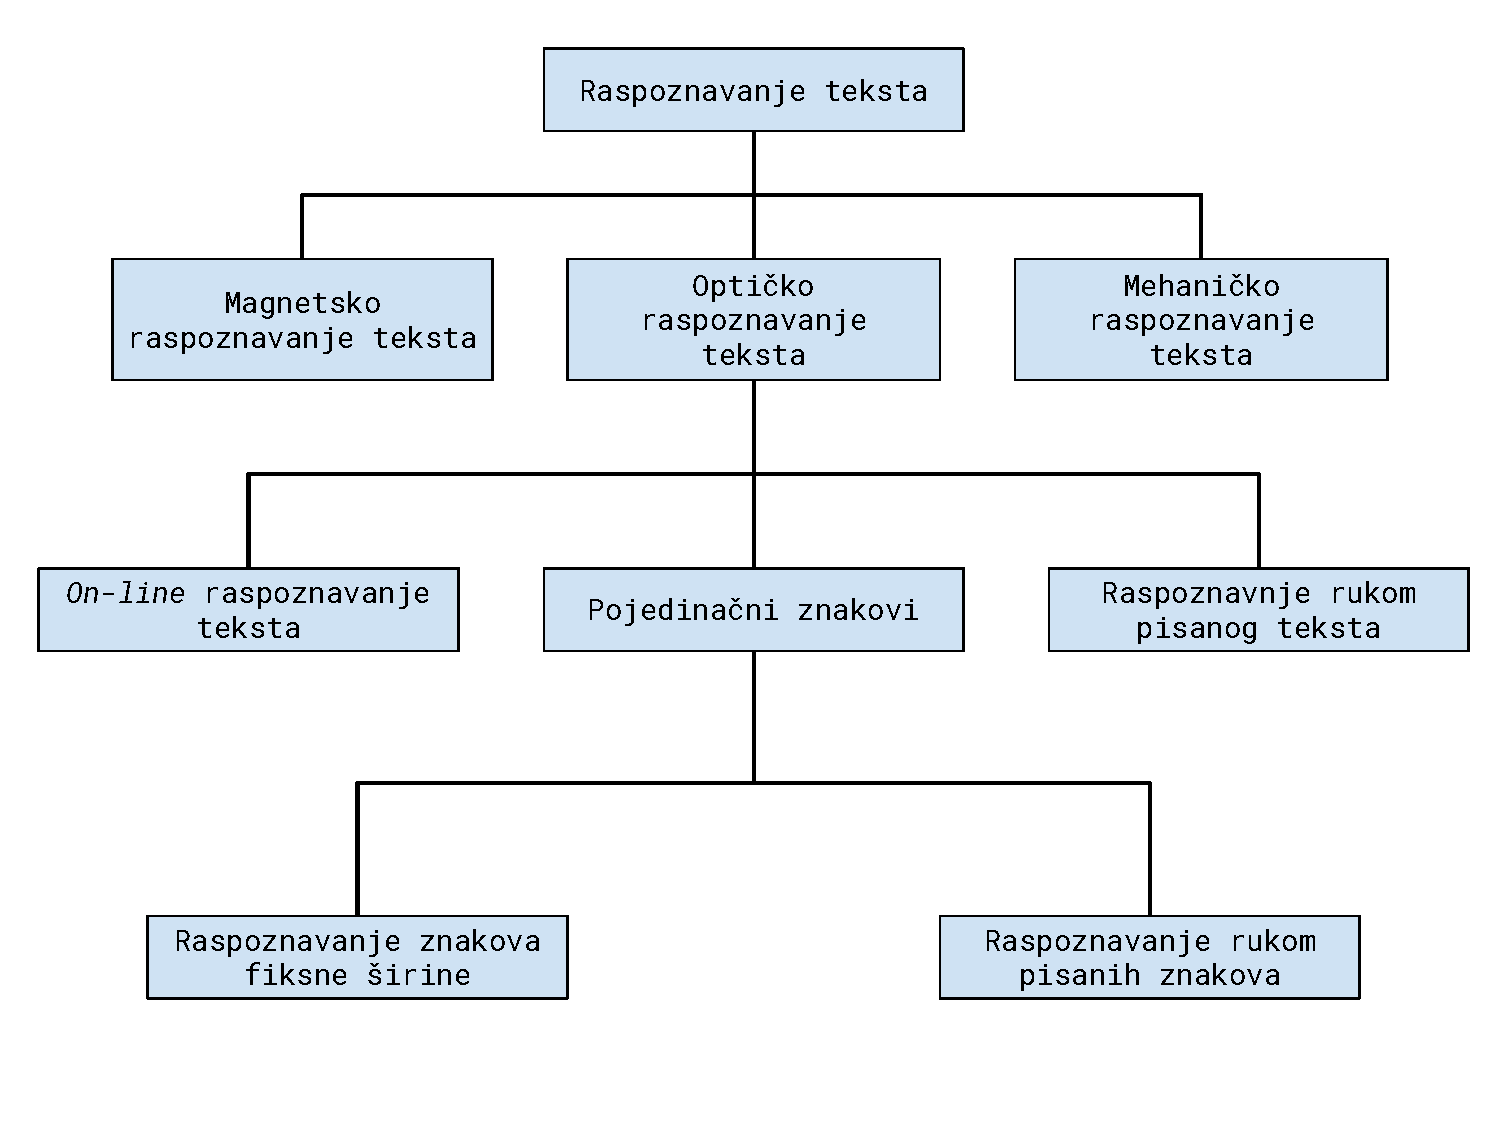
\includegraphics[width=12cm]{images/character-recognition-categories.pdf}
    \caption{Podjela područja raspoznavanja teksta.}
    \label{fig:podjela-podrucja-raspoznavanja-teksta}
\end{figure}

S obzirom na korištene značajke, tehnike raspoznavanja teksta možemo razvrstati u dvije
kategorije\ \citep{govindan1989}:
\begin{enumerate}
    \item \emph{Tehnika korelacije i podudaranja predložaka}
    \item \emph{Tehnika analize i podudaranja značajki}
\end{enumerate}
Kod tehnike korelacije i podudaranja predložaka ulazni znakovi se uspoređuju sa skupom predložaka znakova te se
klasifikacija obavlja na temelju sličnosti. Metoda usporedbe znakova može biti veoma jednostavna, kao što je usporedba
svakog pojedinog odgovarajućeg piksela, ili komplicirana, kao na primjer usporedba koristeći stablo odluke koje određuje
koji pikseli će se uspoređivati. Glavni nedostatak ove tehnike je neotpornost na ulazne smetnje i varijaciju u stilu
pisanja. Tehnika analize i podudaranja značajki češće je korištena tehnika raspoznavanja teksta. Ova tehnika
podrazumijeva odabir odgovarajućih značajki koje se uspoređuju sa značajkama idealnih znakova te se znak čije se
značajke najviše podudaraju s ulaznim primjerom dodjeljuje kao prepoznati znak\ \citep{govindan1989}.


\section{Pristupi problemu raspoznavanja teksta}
\label{sec:pristupi-problemu-raspoznavanja-teksta}
U području raspoznavanja uzoraka postoje dva glavna pristupa: prvi pristup je statistički ili teoretski pristup, a drugi
pristup je sintaktički ili strukturni pristup\ \citep{govindan1989}. Svaki od navedenih pristupa ima svoje prednosti i
mane. Na primjer, kod kompleksnih uzoraka statistički pristup ne može dovoljno precizno opisati informacije o međusobnim
strukturnim vezama između komponenti te time gubi na preciznosti pri raspoznavanju. S druge strane, sintaktički pristup
ne može u potpunosti opisati ulazne uzorke na temelju strukturnih modela znakova. Uzorci su prirodne pojave koje se ne
mogu uvijek u potpunosti opisati matematičkim i formalnim jezikom. Zbog toga, za raspoznavanje teksta potrebne su
tehnike za opisivanje velikog broja sličnih struktura iste kategorije dok istovremeno dozvoljavamo različite opise
među kategorijski različitim uzorcima\ \citep{govindan1989}. Pristup problemu raspoznavanja znakova također možemo
podijeliti ovisno o korištenoj metodologiji. Metodologije za raspoznavanje teksta mogu se svrstati u sljedećih 6
kategorija\ \citep{mantas1986}:
\begin{enumerate}
    \item \emph{Globalna usporedba točaka} - pikseli ulazne slike uspoređuju se sa svim pikselima baze znakova.
    \item \emph{Globalne transformacije} - kao značajke odabiru se vrijednosti dobivene koristeći neku od globalnih
    transformacija nad ulaznom slikom, kao na primjer \emph{Karhunen-Loèveova} ili \emph{Fourierova} transformacija.
    \item \emph{Odabir lokalnih značajki} - pod ovu kategoriju spadaju značajke dobivene analizom krajnjih točaka
    znakova, točaka presjecišta linija, vrijednosti kuteva među linijama te ostalim sličnim metodama. Često je potrebno
    stanjiti ulazne znakove prije određivanja vrijednosti značajki.
    \item \emph{Odabir značajki koristeći linije} - koriste se vertikalne, horizontalne te dijagonalne linije kako bi
    se odredile vrijednost značajki.
    \item \emph{Analiza krivulja} - značajke se određuju preko smjera krivulja i geometrijske analize.
    \item \emph{Strukturna analiza} - ulazni znakovi rastavljaju se na manje gradivne komponente koje se zatim
    reduciraju u graf koji opisuje topologiju znaka.
\end{enumerate}
Neovisno o odabranoj metodologiji, proces raspoznavanja teksta može se ugrubo podijeliti u tri dijela: pretprocesiranje,
odabir značajki te klasifikacija\ \citep{mori1999}. Pretprocesiranje je korak je čija se važnost često zanemari u odnosu
na preostala dva koraka, ali ono je podjednako važno. Kvalitetno pretprocesiranje može značajno smanjiti kompleksnost
ulazne slike te time olakšati proces odabira značajki, što će dalje pridonijeti boljoj klasifikaciji.


\section{Analiza postojećih radova}
\label{sec:analiza-postojecih-radova}
Ovaj rad bavi se raspoznavanjem rukom pisanih znamenaka, koje je podskupom problema raspoznavanja ručno pisanog teksta.
Raspoznavanje rukom pisanog teksta podrazumijeva da ne postoje ograničenja stila pisanja i odvojivosti
znakova\ \citep{mantas1986}. Ovaj odjeljak analizira nekoliko znanstvenih radova koji nude razne pristupe navedenom
problemu.

\subsection{Raspoznavanje rukom pisanih znamenki koristeći unaprijednu neuronsku mrežu}
\label{subsec:raspoznavanje-rukom-pisanih-znakova-koristeci-unaprijednu-neuronsku-mrezu}
Postupak opisan u\ \citep{leCun1990} koristi unaprijednu neuronsku mrežu uz minimalno pretprocesiranje. Glavni cilj rada
bio je pokazati da se unaprijedna neuronska mreža može koristiti za raspoznavanje znamenaka bez korištenja kompleksnog
pretprocesiranja ulaznih slika. Stoga je ulaz neuronske mreže cijela slika umjesto vektora značajki. Time je pokazana
mogućnost unaprijedne neuronske mreže da uspješno interpretira informacije niske razine te uz pomoć njih klasificira
ulaznu sliku. Pošto je ulaz neuronske mreže fiksne veličine, sve slike su skalirane na veličinu $16 \times 16$
piksela\footnote{Prosječna veličina slike bila je $40 \times 60$ piksela.} koristeći linearnu transformaciju. Slike su
pri skaliranju zadržale svoj originalan omjer visine i širine, pa zbog toga nastaju sive nijanse koje se normaliziraju
na raspon $[-1, 1]$ koji se koristi kao ulazna vrijednost neuronske mreže. Korištena neuronska mreža ima 10 izlaza, sa
željenim izlaznim vrijednostima u rasponu $[-1, 1]$. Kako arhitektura neuronske mreže jako utječe na njenu sposobnost
generalizacije, bilo je potrebno uvesti ograničenja za vrijeme postupka učenja kako bi se izbjegla prenaučenost mreže.
Prvo ograničenje nalazi se u početnim slojevima mreže tako da neuroni u tim slojevima mogu tvoriti međusobne veze
samo lokalno. Na ovaj način dobivaju se izlazi koji će biti ekvivalentni konvoluciji s malom jezgrom i funkcijom
sažimanja. Ostatak mreže koristi sličan princip ograničenja veza među neuronima, ali također uvodi lokalno
ujednačavanje. Time je postignuta otpornost mreže na translacije i ulazne smetnje u slici.\\
\begin{figure}[htb]
    \centering
    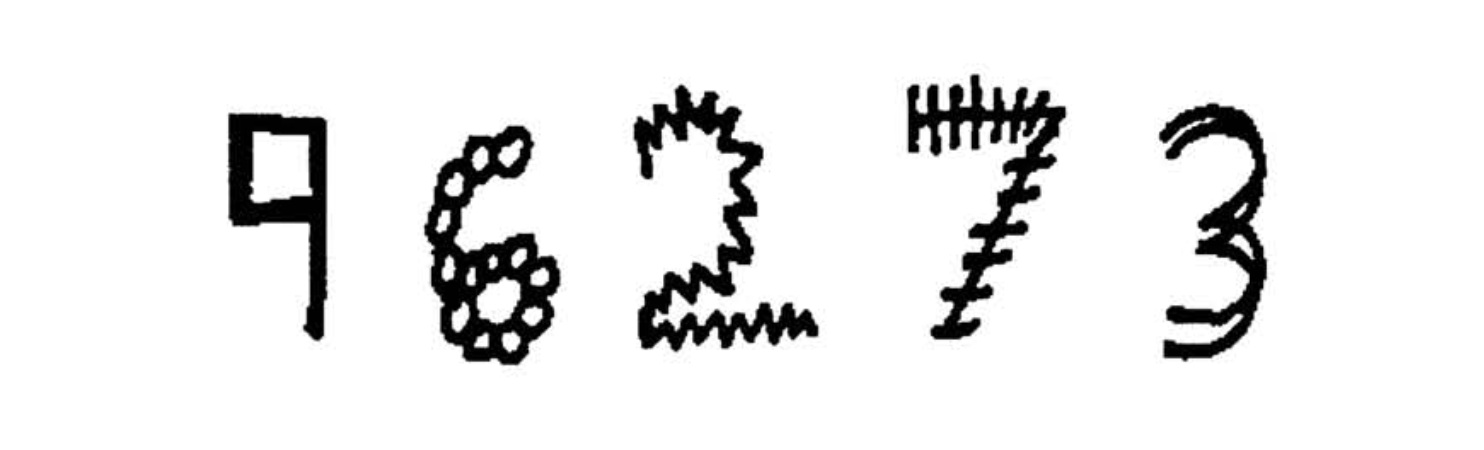
\includegraphics[width=12cm]{images/atypical-data.png}
    \caption{Atipično stilizirane znamenke.}
    \label{fig:atipicno-stilizirane-znamenke}
\end{figure}
Segmentacija slika je obavljena ručno te rad ne razmatra postupak segmentacije. Korišteni skup podataka sastoji se od
9298 rukom pisanih brojeva i 3249 tiskanih brojeva koristeći 35 različitih fontova. Skup za učenje koristio je 7291
rukom pisanih i 2549 tiskanih brojeva dok je testni skup sadržao preostalih 2007 rukom pisanih i 700 tiskanih brojeva.
Fontovi korišteni u skupu za učenje i testnom skupu su različiti. Postignuta greška na skupu za učenje iznosi $1.1\%$
dok greška na testnom skupu iznosi $3.4\%$. Sve pogreške klasifikacije dogodile su se na podskupu rukom pisanih znakova.
Naučena mreža također uspješno raspoznaje atipično stilizirane znamenke, kao što je prikazano na
slici\footnote{Slika je preuzeta iz\ \citep{leCun1990}.}\ \ref{fig:atipicno-stilizirane-znamenke}.

\subsection{Raspoznavanje rukom pisanih znakova koristeći lokalne gradijente opisnika značajki}
\label{subsec:raspoznavanje-rukom-pisanih-znakova-koristeci-lokalne-gradijente-opisnika-znacajki}
Metoda lokalnih gradijenata kao odabranih značajki znakova pokazuje bolje rezultate nego metode koje direktno koriste
intenzitete piksela kao ulaze kao što je pokazano u\ \citep{surinta2015}. Navedeni rad analizirao je raspoznavanje
znakova i brojeva koristeći metodu lokalnih gradijenata na tri različita pisma: Latiničnom, Tajlandskom i Bengalskom.
Rad opisuje dva pristupa računanju lokalnih gradijenata: prvi pristup koristi histogram orijentiranih gradijenata
(\emph{HOG}) dok drugi pristup koristi transformaciju značajki koja ne ovisi o veličini (\emph{SIFT}\footnote{
    \emph{Engl. scale invariant feature transform.}}).\\
Kod pristupa \emph{HOG}, ulazne značajke definiraju se kao distribucija intenziteta lokalno orijentiranih gradijenata
slike koji se računaju za male povezane regije. Za svaki piksel slike računaju se sljedeće vrijednosti:\\
\\
$G_x = f(x + 1, y) - f(x - 1, y)$\\
$G_y = f(x, y + 1) - f(x, y - 1)$\\
\\
$G_x$ je horizontalna, a $G_y$ vertikalna komponenta gradijenta u nekom pixelu $(x, y)$. Ulazni raspon za smjer
gradijenta ograničen je na $[0^{\circ}, 180^{\circ}]$. Magnituda gradijenta $M$ i smjer gradijenta $\alpha$ računaju se
na sljedeći način:\\
\\
$M(x, y) = \sqrt{{G_x}^2 + {G_y}^2}$\\
$\theta(x, y) = \arctan{\frac{G_y}{G_x}}$\\
\\
Nakon ovog koraka, histogrami se računaju iz vrijednosti usmjerenih gradijenata za blokove određene veličine.
Kombinacija histograma svih blokova tvori vektor ulaznih značajki. Pokazano je kako performansa ovakvog opisnika ovisi
o broju blokova u ulaznoj slici, tako da je potrebno pažljivo odabrati veličinu bloka u odnosu na veličinu slike. Prije
korištenja dobivenog vektora značajki, provodi se njegova normalizacija koristeći L2 normu:\\
\\
${V_k}^{'} = \frac{V_k}{\sqrt{{||V_k||}^2 + \epsilon}}$\\
\\
$V_k$ je kombinirani histogram svih blokova, $\epsilon$ je mala konstanta blizu nule, a ${V_k}^{'}$ je normalizirani
vektor značajki.\\
Pristup \emph{SIFT} računa $128$-dimenzijski vektor značajki za određene ključne točke slike. Kako broj ključnih točaka
može varirati ovisno o ulaznoj slici, u radu je odabran određen broj fiksnih ključnih točaka, kao na primjer sredina
ulazne slike. Metoda \emph{SIFT} prvo računa vrijednost konvolucije koristeći \emph{Gaussovu} jezgru varijabilne
veličine:\\
\\
$L(x, y, \sigma) = G(x, y, \sigma) * I(x, y)$\\
\\
$I(x, y)$ je intenzitet piksela $(x, y)$, a $G(x, y, \sigma)$ je \emph{Gaussova} jezgra. Parametar $\sigma$ odrađuje
širinu \emph{Gaussove} jezgre. Nakon toga računaju se horizontalne i vertikalne komponente gradijenta:\\
\\
$G_x = L(x + 1, y, \sigma) - L(x - 1, y, \sigma)$\\
$G_x = L(x, y + 1, \sigma) - L(x, y - 1, \sigma)$\\
\\
Zadnji korak ove metode računa magnitude i smjerove gradijenata na isti način kao i kod metode \emph{HOG}. Kao
klasifikatori korišteni su algoritam $k$-najbližih susjeda i stroj potpornih vektora. Skup za treniranje sastoji se od
preko 60 tisuća znakova, dok se testni skup sastoji od oko 17 tisuća znakova kroz sva tri korištena pisma. Kod
klasifikacije algoritmom $k$-najbližih susjeda metoda \emph{SIFT} pokazuje znatno bolje rezultate na Tajlandskom i
Bengalskom skupu znakova, dok metoda \emph{HOG} dalje bolje rezultate za Latinične znakove. Međutim, klasifikacija
strojem potpornih vektora daje najbolje rezultate za sva tri pisma koristeći metodu \emph{SIFT}.

\subsection{Segmentacija i raspoznavanje teksta na kompleksnoj pozadini temeljeno na Markovljevom nasumičnom polju}
\label{subsec:segmentacija-i-raspoznavanje-teksta-na-kompleksnoj-pozadini-temeljeno-na-markovljevom-nasumicnom-polju}
Većina metoda za raspoznavanje teksta koristi pretpostavku da je raspodjela sivih nijansi ulazne slike bimodalna te da
su znakovi isključivo crni ili bijeli dijelovi te razdiobe. Postupak opisan u\ \citep{chen2002} razmatra raspoznavanje
znakova na kompleksnoj pozadini gdje je moguće da su sive nijanse znakova jako slične sivim nijansama pozadine. U tom
slučaju pokazano je da klasifikacija može jako varirati ovisno o kvaliteti segmentacije ulazne slike pošto se greške
segmentacije direktno prenose u postupak klasifikacije. Navedeni postupak stoga generira određeni broj hipoteza o
segmentaciji slike kod kojih se zatim provodi analiza povezanih komponenti. Svaka hipoteza šalje se dalje u klasifikator
koji dalje vjerojatnosnu vrijednost klasifikacije te se odabire najvjerojatniji rezultat. Kod postupka segmentacije
intenziteti ulaznih piksela modeliraju se kao kombinacija $K$ nasumičnih procesa. Svaki nasumični proces može se
smatrati jednim slojem ulazne slike koji sadrži slične vrijednosti intenziteta, te će jedan od njih sadržavati ulazne
znakove. Rad je testirao dva algoritma za proces segmentacije: \emph{EM}\footnote{Algoritam maksimizacije očekivanja,
    \emph{engl. Expectation-maximization algorithm}.} i \emph{GEM}\footnote{\emph{Gibbsov} algoritam maksimizacije
očekivanja.}. Kod \emph{EM} algoritma, kombinacija svih nasumičnih procesa definira se na sljedeći način:\\
\\
$p(o_s) = \sum_{k = 1}^{K} p(o_s | e_s = k) p(e_s = k) = \sum_{k = 1}^{K} \pi_k p_k(o_s)$\\
\\
Koristeći normalnu razdiobu $p_i(o_s) = \mathcal{N}(\mu_i, \sigma_i)$, potrebno je pronaći skup parametara
$(\mu_i, \sigma_i, \pi_i)$ za koji područje oznaka $e = \{e_s, 1 \leq e_s \leq K, s \in S\}$ najbolje opisuje ulazne
vrijednosti intenziteta piksela. Slika je definirana preko intenziteta piksela $o = \{o_s, s \in S\}$ gdje $o_s$
označava intenzitet pojedinog piksela dok je $S$ skup svih piksela slike. Algoritam \emph{GEM} poboljšava navedeni
postupak modeliranjem nasumičnih procesa kao \emph{Markovljevih} nasumičnih polja te se umjesto odabira parametara s
najvećom vjerojatnošću provodi optimizaciju maksimalne aposteriorne vjerojatnosti.\\
Nakon pronalaženja optimalnih parametara, nad svakim dobivenim slojem provodi se analiza povezanih komponenti. Svaki
sloj smatra se jednom binariziranom slikom koja se dalje šalje na postupak klasifikacije. Stoga je izbor vrijednosti
$K$ također bitan dio kod ovakvog pristupa raspoznavanju\footnote{U radu su korištene vrijednosti $K \in [2, 4]$.}.
